\chapter{Analýza}

V~tejto kapitole si na~základe potrieb vyplývajúcich z~návrhu užívateľského rozhrania (viď~kap.~\ref{navrh ui}) rozhodneme, aké technológie a prístupy sa nám hodia na~implementáciu systému, a~teda aké využijeme.

\section{Výber typu aplikácie}

Kvôli požiadavke P10~(Dostupnosť, viď v~podkap.~\ref{poziadavky}) dáva dobrý zmysel vytvoriť náš systém ako webovú aplikáciu~-- vyriešime tým problém s~distribúciou softvéru k~(aj potenciálne novým) zákazníkom. Statická stránka by nám nestačila nakoľko chceme administrátorom umožniť dynamickú zmenu obsahu (napr.~pridávanie alebo~mazanie bagrov, prídavných zariadení atď.).

\section{Rozdelenie na~frontendovú a~backendovú časť}
\label{rozdelenie na frontendovu a backendovu cast}

Kvôli lepšej organizácií kódu dáva pre~našu aplikáciu dobrý zmysel rozdeliť ju na~frontendovú a~backendovú časť. Frontendová časť pokryje užívateľské rozhranie navrhnuté v~kap.~\ref{navrh ui} a~backendová časť pokryje zbytok logiky systému (napr.~prácu s~databázou, aukčný odpočet atď.).

V~súčasnosti rôzne spoločnosti, napr. Amazon alebo~Cloudflare, poskytujú backendové služby, tzv.~Backend-as-a-Service~(Baas)~\cite{baas}. Ak by sme sa rozhodli využiť takúto službu, ušetrilo by nám to implementovanie užívateľskej autentifikácie (vyžadované požiadavkou~P6) alebo~práce s~databázou (vyžadované napr.~požiadavkou~P2.4). Ale ak by sme chceli naimplementovať napr.~vyhodnocovanie aukcie alebo~funkcionalitu, ktorá umožní meniť administrátorovi formát automaticky generovaných správ týkajúcich sa aukcie (vyžadované v~požiadavkách~P4 a~P5.3), tak BaaS by nám na~to nestačil. Navyše ak spoločnosť neposkytuje bezplatnú možnosť využívania BaaS, využitie BaaS by bolo v~rozpore s~požiadavkou~P11. Kvôli týmto dôvodom si budeme musieť naimplementovať vlastnú backendovú časť.

Pre~implementáciu backendovej časti by sa mohli hodiť vysokoúrovňové jazyky, akými sú napr.~Java alebo~C\#. Nakoľko ide o podobné jazyky a autor jazyk Java neovláda, ale C\# áno, tak si volíme C\# a~platformu~.NET, ktorá je s~ním spojená.

V~prípade frontendovej časti je zvyčajnou voľbou jazyk~JavaScript (príp.~TypeScript), a~keďže s~ním už má autor nejaké skúsenosti, tak predstavuje jednu z~možností. No v~súčasnosti je možné využiť aj vo~frontendovej časti jazyk C\#. Ako už bolo spomenuté, autor tento jazyk pozná. Navyše ak by sme si vybrali C\#, tak by to znamenalo, že frontendová aj backendová časť, by boli obe napísané v~rovnakom jazyku, čo by mohlo viesť k~zjednodušeniu implementácie. A~preto je C\# ďalšou z~možností jazykov, ktoré môžeme využiť vo~frontendovej časti. Obe jazyky so~sebou prinášajú svoje frontendové frameworky, ktoré nám dokážu uľahčiť implementáciu frontendovej časti. V~následujúcej podkapitole sa pozrieme na~možné typy webovej aplikácie a~frameworky, ktoré môžme využiť na~ich implementáciu. Podľa toho si vyberieme jazyk pre~frontendovú časť.

\section{Výber typu webovej aplikácie}
\label{vyber typu webovej aplikacie}

V~predchádzajúcej podkapitole sme si rozdelili aplikáciu na~frontendovú a~backendovú časť. Takisto sme si predstavili jazyky, ktoré by sme mohli v~týchto častiach využiť. Každý jazyk so~sebou nesie i~svoje frameworky. V~tejto podkapitole sa pozrieme na~to, aký typ webovej aplikácie by mal byť náš systém a~podľa toho si aj zvolíme jazyk s~frameworkom.

\subsection{Single-page application}
\label{single page application}

Single-page application~(SPA)~\cite{spa} je druh webovej aplikácie, ktorá po~príchode užívateľa na~stránku načíta jeden webový dokument, a~potom už iba mení jeho obsah. Väčšina logiky aplikácie sa vykonáva na~strane klienta, preto je aplikácia veľmi rýchla z~hľadiska interakcie s~užívateľom.

Ako už bolo skôr spomenuté, naša aplikácia mení obsahovú časť podľa toho, v~akej sekcii sa užívateľ nachádza (viď~\ref{hlavne rozlozenie aplikacie}). Takisto v~sekcii~,,Správa webu`` preklikávaním medzi kartami sa mení obsah, ktorý vidí užívateľ (spomenuté v~\ref{splnenie p5 p7 a sprava predmetov}). Podobne na~stránkach s~formulármi (detail bagra, prídavného zariadenia, aukčnej podnuky alebo~sekcia Služby) chceme umožniť zobrazovanie a~schovávanie formulára (spomenuté v~\ref{detail bagra pridavneho zariadenia}, \ref{detail aukcnej ponuky} a~\ref{splnenie p8}). Aj kvôli týmto dôvodom sa zdá, že voľba SPA by bola rozumná.

Jazyk JavaScript (resp.~TypeScript) nám ponúka viacero frontendových frameworkov pre~tvorbu SPA aplikácií, napr.~AngularJS, ReactJS, Vue atď. Systém by sa dal naimplementovať ktorýmkoľvek z týchto frameworkov, no kvôli predošlej skúsenosti autora si ako zástupcu JavaScriptových frameworkov zvolíme ReactJS. Ďalej jazyk C\# nám ponúka framework Blazor WebAssembly.

Obe frameworky, ReactJS aj Blazor WebAssembly, fungujú na~princípe komponentov. Komponent si môžeme predstaviť ako nejakú ucelenú časť stránky, napr.~tlačidlo, formulár, navigácia atď. Akonáhle je komponent zadefinovaný, môže sa využívať vo~viacerých častiach webu. Všimnime si, že v~našom návrhu užívateľského rozhrania sa nachádza viacero častí, ktoré vyzerajú úplne rovnako (príp.~sú rozdiely minimálne, ale to sa dá vyriešiť parametrizáciou komponentov), napr.~formuláre v~časti s~detailami bagra, prídavného zariadenia alebo~v~sekcii~Služby (viď~pravú stranu obrázkov~\ref{detail bagra pridavneho zariadenia}, \ref{detail aukcnej ponuky}, \ref{splnenie p8}).

Zatiaľ sa zdá, že obe frameworky by boli dobrou voľbou. No použitie SPA prístupu by nám takisto prinieslo zopár nevýhod:

\begin{itemize}
\item \textbf{Prvotný čas načítania stránky}

Ako bolo spomenuté, väčšina logiky aplikácie sa vykonáva na~strane klienta, kvôli tomu sa pri~prvotnom načítaní stránky sťahujú zdrojové kódy aplikácie, a~to spôsobuje zdržanie. Toto správanie by mohlo odradiť nových potenciálnych zákazníkov.

\item \textbf{SPA nie sú ,,SEO-friendly``}

Search engine optimization~(SEO)~\cite{seo} je proces optimalizovania stránky na~to, aby bola jednoducho dohľadateľná vyhľadávačmi (search engines). Vyhľadávače, akým je napr.~Google, prechádzajú stránky na internete, hodnotia ich a~na základe toho vedia usúdiť, či je stránka pre užívateľa relevantná.

V~prípade SPA aplikácii nastáva problém, pretože obsah je užívateľom generovaný dynamicky a~vyhľadávače majú pri~prechádzaní s~týmto správaním SPA aplikácií problém. Nie je síce nemožné vytvoriť ,,SEO-friendly`` SPA aplikáciu, ale ide o~komplikovanejší proces. Viac informácii na túto tému môžeme nájsť na stránkach Novateus~\cite{novateus} a~Cloudways~\cite{cloudways}.

\item \textbf{Potenciálny problém so~staršími verziami prehliadačov}

Tento bod sa vzťahuje skôr špeciálne k Blazor WebAssembly. Aktuálne verzie prehliadačov obsahujú všetky nástroje potrebné pre~bezproblémový beh SPA aplikácií (resp. podporujú technológiu web assembly). Avšak ako bolo spomenuté v~požiadavke P10 (Dostupnosť, viď~v~podkap.~\ref{poziadavky}), hrozí, že firemné počítače môžu využívať staré verzie prehliadačov, na~ktorých by SPA aplikácie nemuseli fungovať správne. Táto myšlienka vychádza z toho, že v prehliadači Google Chrome (ktorý je v~roku~2023 podľa štatistík najpopulárnejším prehliadačom~\cite{stats}) nebola technológia web assembly vôbec podporovaná do verzie 50~\cite{wa support} a~najvyššia podporovaná verzia priehliadača Google Chrome na~počítačoch s~operačným systémom Windows XP neprevyšuje verziu 50~\cite{chromexpver1}~\cite{chromexpver2}~\cite{chromexpver3}.
\end{itemize}

\subsection{Multi-page application}
\label{multi page application}

Multi-page application~(MPA)~\cite{mpa} je druh webovej aplikácie, ktorá využívia klasický prístup~-- keď užívateľ klikne na~nejaký odkaz, odošle sa serveru žiadosť, a~ten vráti užívateľovi ako odpoveď celú stránku. Väčsina logiky aplikácie sa vykonáva na~serveri a~užívateľovi sa podáva iba HTML, CSS a JavaScript.

Autorovi sa nepodarilo nájsť žiadne JavaScriptové MPA frameworky, ale~v~prípade jazyka~C\# je známym ASP.NET MVC~\cite{aspnetmvc}. Ak by sme si zvolili tento framework, a teda využili MPA prístup, tak pri preklikávaní odkazmi navigácie by každá zmena obsahovej časti aplikácie (viď~\ref{hlavne rozlozenie aplikacie}) síce znamenala načítanie novej stránky, ale to by nepredstavovalo problém. Takisto by sa dali pomocou frameworku ASP.NET MVC naimplementovať stránky s formulármi (detail bagra, prídavného zariadenia, aukčnej podnuky alebo~sekcia Služby) a aj prepínanie medzi kartami v~sekcii~,,Správa webu`` (spomenuté v~\ref{splnenie p5 p7 a sprava predmetov}).

Takže sa zdá, že aj implementácia pomocou MPA prístupu je možná a navyše má oproti SPA výhody:

\begin{itemize}
\item \textbf{Prvotný čas načítania stránky}

Narozdiel od~SPA sa väčšina logiky vykonáva na~serveri, kde sú aj uložené zdrojové kódy aplikácie, kvôli tomu si ich užívateľ nemusí sťahovať k~sebe a~prvotné načítanie stránky nie je pomalé.

\item \textbf{MPA sú \uv{SEO-friendly}}

Vyhľadávače, akým je napr. Google, nemajú problém pri~prechádzaní obsahu takýchto aplikácií. Preto sú MPA aplikácie \uv{SEO-friendly}.

\item \textbf{Neexistuje problém so~staršími verziami prehliadačov}

Kedže sa užívateľom podáva iba HTML, CSS, príp. JavaScript, a teda nie je nutné spúšťať kód typu web assembly, tak ani staršie verzie prehliadačov by nemali mať problém s behom aplikácie. Takže nedochádza k porušeniu požiadavky P10 (viď~\ref{poziadavky}).
\end{itemize}

To boli výhody oproti SPA aplikáciam, ale MPA aplikácie majú takisto nevýhody:

\begin{itemize}
\item \textbf{Záťaž vyvíjaná na server}

Ako bolo spomenuté, užívateľ každým kliknutím na odkaz odosiela žiadosť na server, ktorú musí server spracovať a následne odoslať odpoveď~-- to vyvíja záťaž na server. V prípade veľkého množstva užívateľov by to mohlo predstavovať problém, ale my vytvárame aplikáciu pre malé firmy, kde sa nepredokladá obrovské množstvo pripojení v rovnakú chvíľu. Takže táto nevýhoda je pre nás nepodstatná.

\item \textbf{Absencia komponent}

V predošlej časti textu bolo spomenuté, že jednou z výhod frameworkov ReactJS a Blazor WebAssembly je koncept komponentov. V prípade ASP.NET MVC tento koncept chýba, alebo presnejšie, nie je natívne podporovaný, ale dá sa napodobniť~\cite{components in aspnet mvc}. Takže napríklad implementácia časti s preklikovateľnými kartami (\ref{splnenie p5 p7 a sprava predmetov}) alebo častí, ktoré sú totožné, napr.~formuláre v~časti s~detailami bagra, prídavného zariadenia alebo~v~sekcii~Služby (viď~pravú stranu obrázkov~\ref{detail bagra pridavneho zariadenia}, \ref{detail aukcnej ponuky}, \ref{splnenie p8}) by sa dala realizovať i bez duplicitného kódu, ale nebolo by to až tak prehľadné ako v spomínaných frameworkoch, ktoré podporujú koncept komponentov nativne.
\end{itemize}

Zdá sa, že MPA aplikácie by vyriešili nejaké z nevýhod SPA aplikácii, ale takisto nie sú dokonalé a nesú so sebou nejaké nevýhody, ktoré však pre nás nie sú príliš podstatné. Preto by sa zdalo, že MPA je prístup, ktorý by sme mali využiť. Existuje však ešte jedna alternatíva, a tou je Blazor Server, o ktorom si povieme v následujúcej časti textu.

\subsection{Blazor Server}

Blazor Server~\cite{blazor server} je framework jazyka C\# a~je to framework na vývoj webových aplikácií, ktoré sú ,,tak niečo medzi`` SPA a MPA aplikáciami. Väčšina kódu aplikácie sa vykonáva na serveri ako v prípade MPA aplikácií. Rozdiel je v tom, že ak na strane klienta dôjde k zmene nejakej časti užívateľského rozhrania, tak namiesto toho, aby server odoslal klientovi celú stránku, odošle iba potrebné zmeny. To umožňuje vytváranie interaktívneho užívateľského rozhrania ako v prípade SPA aplikácií.

Ak by sme využili Blazor Server na vývoj našej aplikácie, tak by mala naša aplikácia rovnaké výhody ako má MPA aplikácia oproti SPA aplikácii (viď~časť~\ref{multi page application}). No navyše oproti MPA aplikácii by mala výhody:

\begin{itemize}
\item \textbf{Existencia komponentov}

V SPA časti bolo v súvise s frameworkmi ReactJS a Blazor WebAssembly spomenuté, že koncept komponentov by sa nám v našej aplikácii hodil (viď~časť~\ref{single page application}). Potom v časti MPA sme spomenuli, že ASP.NET MVC by nám síce umožňil využívať koncept komponentov, ale natívne tento koncept nepodporuje a implementácia by nebola taká jednoduchá, priamočiara ako v prípade frameworkov, ktoré tento koncept podporujú natívne (viď~\ref{multi page application}). Našťastie je Blazor Server jeden z~frameworkov, ktorý tento koncept komponentov natívne podporuje.
\end{itemize}

Je síce pravda, že aj naďalej ostáva nevýhodou vyťažovanie servera ako tomu bolo v prípade MPA aplikácií, ale ako bolo napísané v prechadzajúcej časti textu (viď~časť~\ref{multi page application}), táto nevýhoda pre nás nepredstavuje problém. Navyše výberom tohto frameworku budeme môcť písať aj frontendovú, aj backendovú časť v rovnakom jazyku, čo by mohlo zjednodušiť implementáciu. Preto si volíme ako frontendový jazyk C\# s frameworkom Blazor Server.

\section{Voľba databázy}
\label{volba databazy}

Z požiadaviek na systém vyplýva, že budeme potrebovať databázu pre~uloženie dát (napr. pre uloženie ponuky bagrov, viď požiadavku P2 v~podkap.~\ref{poziadavky}). Typicky sa databázy rozdeľujú na~dva druhy~-- tradičné relačné databázy alebo~alternatívne nerelačné, tzv.~NoSql, databázy.

\begin{itemize}
\item \textbf{Relačné databázy~\cite{relational db}}

Ide o typ databáz, ktorý ukladá a usporiadáva dátové body s~definovanými reláciami pre rýchly prístup. Relačné databázy usporiadávajú dáta do~tabuliek, ktoré obsahujú informácie o~jednotlivých entitách a~predstavujú preddefinované kategórie prostredníctvom riadkov a~stĺpcov. Štruktúrovanie dát týmto spôsobom umožňuje efektivný a~flexibilný prístup. Relačné databázy rozumejú jazyku~SQL, ktorý služí na~ukladanie, načítanie a~manipuláciu s~dátami.

\item \textbf{Nerelačné (NoSql) databázy~\cite{nosql db}}

Tento typ databáz predstavuje databázy \uv{iné než SQL}. Ide o~databázy dokumentové, grafové, key-value atď. Tieto databázy dokážu spracovávať veľké množstvo rýchlo sa meniach neštrukturovaných dát inými způsoby než~relačné databázy s~riadkami a~tabuľkami.
\end{itemize}

NoSql databázy sa hodia pre veľké množstvo neštrukturovaných dát~\cite{nosql pros}. V~našom prípade, kedže vytvárame softvér pre malú firmu, nepredpokladáme veľké množstvo dát (napr.~počet bagrov pravdepodobne nepresiahne sto). Taktiež platí, že štruktúra dát je (v~podstate) predom určená (viď~požiadavky P2.1, P2.2, P2.3 atď. v~podkap.~\ref{poziadavky}). Navyše má  autor trocha viacej skúseností s klasickými relačnými databázami než s~NoSql. Kvôli týmto dôvodom si volíme relačnú databázu.

\subsection{Návrh relačného modelu databázy}
\label{navrh relacneho modelu databazy}

V predchádzajúcej časti textu (viď~\ref{volba databazy}) sme si zvolili relačnú databázu, a~preto bude teraz nasledovať vytváranie relačného modelu databázy~\cite{relational model} (ide o~reprezentáciu dát uložených v~relačnej databáze). Ako už bolo spomenuté v~predchádzajúcej časti textu, štruktúra dát (a~teda aj samotné entity) boli viac-menej zadané už v~podkapitole s~požiadavkami na~systém (viď~\ref{poziadavky}), v~tejto kapitole si upresníme ich formu a~vzťahy medzi nimi (resp.~kardinality). Pre~lepšiu predstavu vytváraného relačného modelu viď~obr.~\ref{relacny model uml}.

\begin{figure}[H]\centering
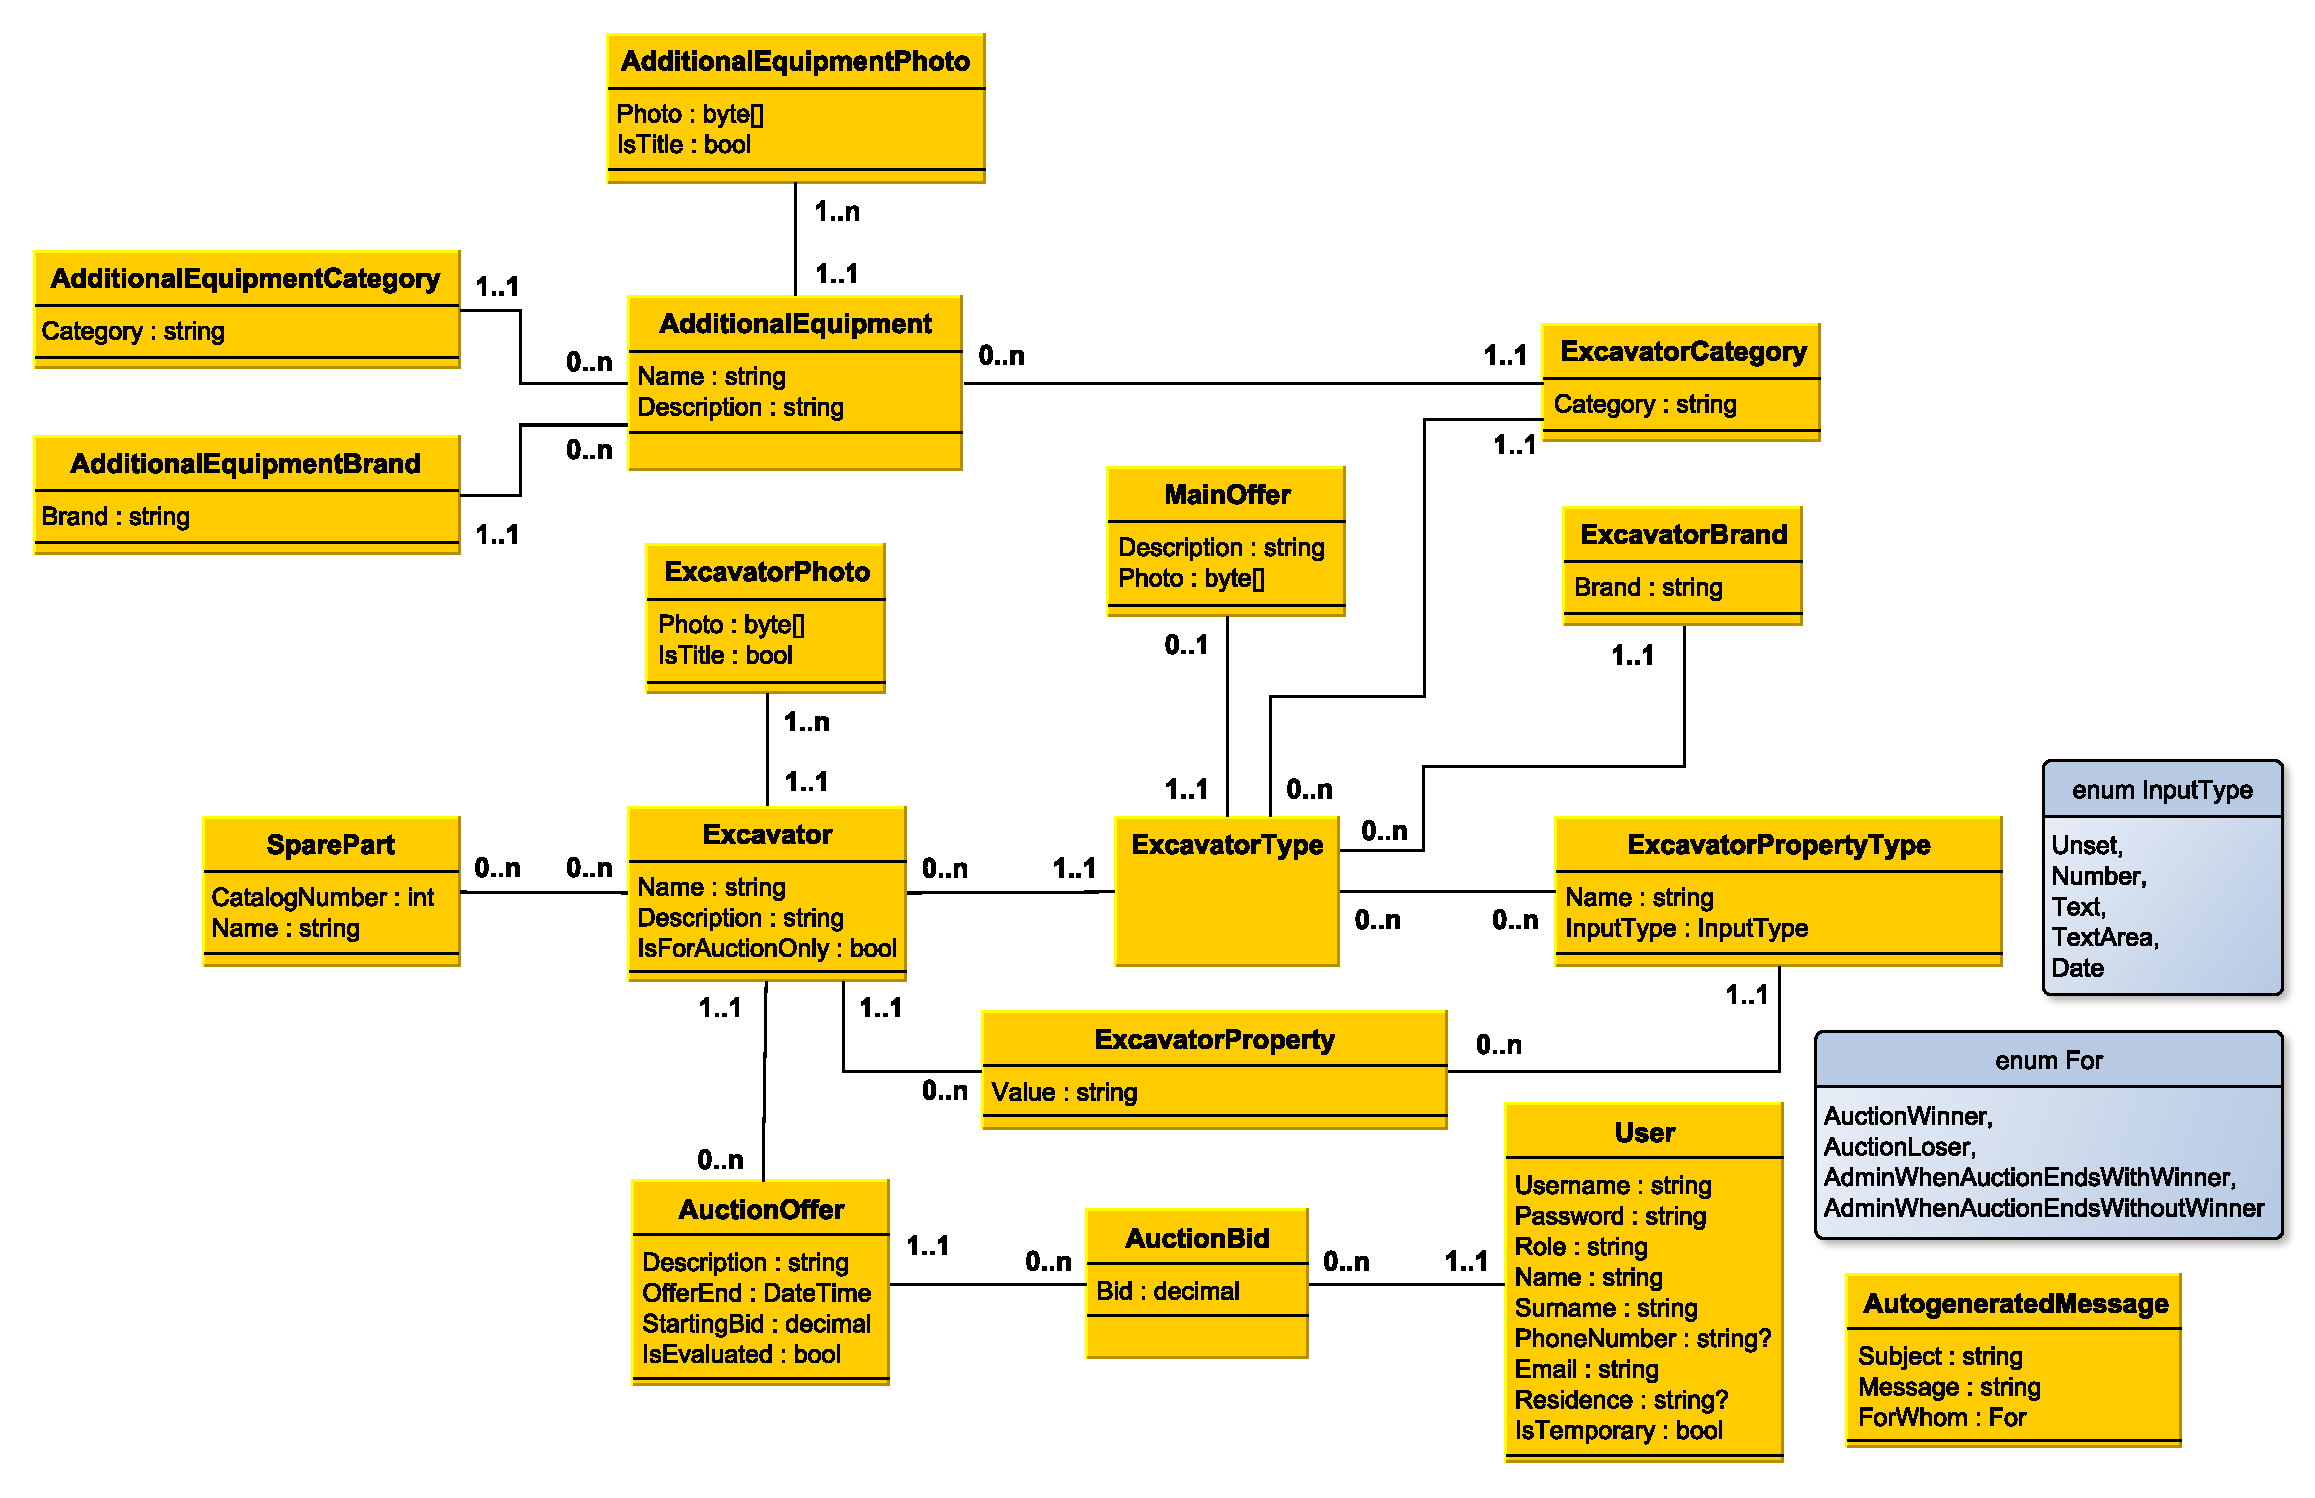
\includegraphics[width=140mm]{../img/relacny model uml}
\caption{Relačný model databázy.}
\label{relacny model uml}
\end{figure}

\begin{itemize}
\item \textbf{Entita Excavator}

V požiadavke P2.2 (Bager, viď~podkap.~\ref{poziadavky}) sme si stanovili, že každý bager má mať názov, značku, kategóriu, opis, fotky, vlastnosti, a~tiež informáciu o~tom, aké náhradné diely obsahuje. Taktiež tam bolo napísané, že môžu existovať bagre, ktoré sú určené iba pre aukciu. To, či je bager určený iba pre aukciu, vieme zachytiť pomocou boolovskej vlastnosti (viď~entitu~Excavator na~obr.~\ref{relacny model uml}). Podobne vieme pomocou vlastností v entite zachytiť aj názov a opis.

\item \textbf{Entita ExcavatorType}

Čo sa týka značky a~kategórie, tak tie by by sme takisto mohli v~entite reprezentujúcej bager zachytiť pomocou vlastností, ale to by znamenalo, že za~každým pri~vytváraní nového záznamu pre bager by sa musela špecifikovať hodnota týchto vlastností. Takisto platí, že viacero bagrov môže byť tej istej kategórie a~značky. Ak by sa mali pri každom vytváraní záznamu bagra vypisovať hodnoty pre značku a kategóriu, mohlo by to viesť k~zbytočným chybám (preklepom), a takisto by to pre administrátora nebolo príliš pohodlné. Preto vytvoríme novú entitu reprezentujúcu typ bagra (viď~ExcavatorType na~obr.~\ref{relacny model uml}), ktorá nám bude určovať kategóriu a~značku bagra. Tato entita však nebude obsahovať vlastnosi ani pre~značku bagra, ani pre~kategóriu bagra.

\item \textbf{Entita ExcavatorBrand a ExcavatorCategory}

Značka bagra, rovnako ako aj kategória bagra, by mali byť novými osobitnými entitami (viď~entity~ExcavatorBrand a~ExcavatorCategory na~obr.~\ref{relacny model uml}), entita reprezentujúca značku bagra by obsahovala vlastnosť s~údajom o~značke bagra a~entita reprezentujúca kategóriu bagra by obsahovala vlastnosť s~údajom o~kategórii bagra. To je z toho dôvodu, že môžu existovať viaceré typy bagra, ktoré by boli rovnakej značky, ale líšili by sa kategóriou (alebo naopak, boli by rovnakej kategórie, ale líšili by sa značkou). Tým, že by sme zo~značky bagra a~kategórie bagra spravili samostatné entity, zamedzili by sme opakujúcim sa hodnotám v~databáze. Takisto kvôli tomuto bude stačiť ak si administrátor v~aplikácii uloží značku (resp.~kategóriu) bagra iba raz, čo môže zamedziť zbytočným chybám (preklepom).

\item \textbf{Entita ExcavatorPhoto}

Tiež boli v súvislosti s bagrami spomenuté fotky bagrov~-- a~tie budú našou ďalšou entitou (viď entitu ExcavatorPhoto na~obr.~\ref{relacny model uml}). Každý bager môže mať viacero fotiek, pričom tieto fotky budeme chcieť zobrazovať napr. v časti aplikácie s detailom bagra, ktorá bola spomenutá v~časti~\ref{detail bagra pridavneho zariadenia} (viď vľavo hore na~obr.~\ref{detail}) alebo~tiež na kartách strojov, ktoré boli spomenuté v~časti~\ref{ponuka novych bagrov} (viď~obr.~\ref{excavator cards}). Entita reprezentujúca fotku bagra by mala okrem samotnej fotky obsahovať aj boolovskú vlastnosť určujúcu, či je fotka titulná. Vďaka tejto vlastnosti budeme môcť presne určiť, aká fotka bagra sa má zobrazovať na~jeho karte.

\item \textbf{Entita SparePart}

Okrem fotiek boli v súvislosti s bagrami spomenuté aj náhradné diely. Náhradný diel bude predstavovať ďalšiu entitu (viď~entitu SparePart na~obr.~\ref{relacny model uml}) a~jeho údaje boli definované v~P7.1~-- má obsahovať katalógové číslo (ide o~celé číslo, neobsahuje iné znaky ako číslice) a~názov náhradného dielu. Každý bager môže obsahovať viacero rôznych náhradných dielov a~jeden náhradný diel sa môže nachádzať vo~viacerých bagroch.

\item \textbf{Entita ExcavatorPropertyType a ExcavatorProperty}

Ďalej boli v súvislosti s bagrami spomenuté aj vlastnosti bagra, ktoré sú určené jeho typom (ako bolo spomenuté v~požiadavke~P2.2). Tu je dôležité uvedomiť si, že typ bagra v skutočnosti určuje typ vlastnosti bagra. Napríklad typ bagra X môže mať vlastnosť hmotnosť a ďalší typ bagra Y môže mať takisto vlastnosť hmotnosť, ale okrem nej môže mať aj vlasnosť šírka lyžice. Všimnime si, že hovoríme o typoch vlastností bagra, ale nie o~konkrétnych hodnotách vlastností, teda napr. koľko vážia bagre typu X, to nemôžeme vedieť, pretože presná hodnota je určená konkrétym bagrom a nie jeho typom. Z toho vyplýva, že budeme potrebovať entitu na reprezentáciu typu vlastnosti bagra (viď entitu ExcavatorPropertyType na obr. \ref{relacny model uml}), ale takisto aj entitu reprezentujúcu (konkrétnu) vlastnosť, ktorá by v sebe niesla konkrétnu hodnotu určenú konkrétnym bagrom (viď entitu ExcavatorProperty na obr. \ref{relacny model uml}). Entita reprezentujúca typ vlastnosti bagra by v sebe mala obsahovať okrem názvu (aby sme vedeli, čo je to za vlastnosť, napr. hmotnosť) aj typ hodnoty danej vlastnosti, aby sme vedeli, či ide o číslo, krátky text, dlhší opis alebo~dátum (s~určením typu hodnoty danej vlastnosti nám pomôže enum~InputType, ktorý môžeme vidieť na~obr.~\ref{relacny model uml}). Tento údaj nám dovolí zlepšiť užívateľské rozhranie, konkrétne typy polí pre hodnoty vlastností bagra vo formulári pre vytvorenie/úpravu bagrov, ktorý bol spomenutý v časti \ref{vytvorenie noveho a uprava existujuceho bagra} (viď obr. \ref{excavator form}).

\item \textbf{Entita MainOffer}

V požiadavke P2 sa vyžaduje, aby existovala aj hlavná ponuka~-- tá bude našou ďalšou entitou (viď entitu MainOffer na obr. \ref{relacny model uml}). Konkrétne v~požiadavke P2.1 sme si stanovili, že hlavná ponuka reprezentuje typ bagrov a~má obsahovať opis, a~tiež fotku danéhu typu. V~predošlom texte bolo spomenuté, že môžu existovať bagre, ktoré by boli určené iba pre~aukciu, a~teda nenachádzali by sa v ponuke (nových) bagrov. Preto môže nastať situácia, kde by sme chceli, aby sa v databáze nachádzal typ bagra, ale~nechceme, aby existovala v databáze hlavná ponuka pre tento typ bagra. Zároveň platí, že hlavná ponuka predstavuje bagre jedného typu.

\item \textbf{Entita AdditionalEquipment}

V požiadavke P2 je tiež spomenutá aj ponuka prídavných zariadení, preto~si vytvoríme aj entitu pre reprezentáciu prídavného zariadenia (viď entitu AdditionalEquipment na obr. \ref{relacny model uml}), tá má podľa požiadavky~P2.3 obsahovať názov, opis, fotky, značku a~kategóriu prídavného zariadenia, ale takisto aj údaj o tom, pre akú kategóriu bagrov je prídavné zariadenie určené. Z~rovnakého dôvodu prečo sme vytvorili novú entitu pre~kategóriu bagra (entita ExcavatorCategory, ktorá bola spomenutá v~prechádzajúcom texte), vytvoríme aj entity reprezentujúce značku prídavného zariadenia (viď~entitu~AdditionalEquipmentBrand na~obr.~\ref{relacny model uml}) a~kategóriu prídavného zariadenia (viď~entitu~AdditionalEquipmentCategory na~obr.~\ref{relacny model uml}). Ďalej čo sa týka fotiek prídavného zariadenia, tak by sa naskytovala možnosť zmeniť entitu reprezentujúcu fotky bagrov (ExcavatorPhoto) na~entitu reprezentujúcu fotky všeobecne (aj bagrov, aj prídavných zariadení). No~tento prístup by nám umožnil priradiť fotku prídavného zariadenia bagru (a~naopak), čo nie je správne. Preto namiesto toho vytvoríme, rovnako ako v~prípade fotky bagra, novú entitu reprezentujúcu fotku prídavného zariadenia (viď~entitu~AdditionalEquipmentPhoto na~obr.~\ref{relacny model uml}).

\item \textbf{Entita User}

Ďalej z požiadavky P6 vieme, že budeme potrebovať entitu reprezentujúcu užívateľa (viď~entitu~User na~obr.~\ref{relacny model uml}). Konkrétne z~P6.3 vieme, že o užívateľovi potrebujeme vedieť jeho prihlasovacie meno, heslo, (krstné) meno, priezvisko, email, príp.~aj telefónné číslo a~bydlisko (mesto). No okrem týchto údajov sa nám tiež kvôli požiadavke P6.1 hodí údaj, či je užívateľ dočasný. Presnejšie je to kvôli tomu, aby aj neprihlásený užívateľ mohol ponúkať sumy do dražby. Po ponúknutí sumy by sa do~databázy uložila informácia o tom, kto ponúkol sumu (a~tiež čo to bolo za~aukčnú ponuku). Po prejdení termínu konca aukčnej ponuky a~vyhodnotení aukcie sa budú môcť tieto dočasné účty vymazať. Okrem toho by sa nám tiež hodil údaj o~tom, či je užívateľ bežným zákazníkom alebo~administrátorom, aby mu podľa toho vedel systém zobraziť správny obsah (vychádza z~P1~Roly užívateľa, viď~podkap.~\ref{poziadavky}). Všetky tieto údaje by mali byť zahrnuté vo~vlastnostiach entity User.

\item \textbf{Entita AuctionOffer}

Z požiadavky P4 vieme, že administrátor by mal byt schopný zaradiť bager do~aukcie a~vytvoriť tak aukčnú ponuku~-- to bude našou ďalšou entitou (viď~entitu~AuctionOffer na~obr.~\ref{relacny model uml}). Takisto z~požiadavky P4 vieme, že administrátor by mal mať možnosť zadať dátum konca aukčnej ponuky, počiatočnú sumu a~popis ponuky (v~ňom môže byť napísané napr.~čo bolo v~bagri opravené). Preto budú tieto údaje vlastnosťami entity~AuctionOffer.

\item \textbf{Entita AuctionBid}

Okrem entity AuctionOffer vyplýva z požiadavky P4 aj entita reprezentujúca ponuku (sumu) ponúknutú zákazníkom (viď~entitu~AuctionBid na~obr.~\ref{relacny model uml}). Údaj o tom, koľko zákazník ponúkol, je vlastnosťou entity~AuctionBid.

\item \textbf{Entita AutogeneratedMessage}

Našou poslednou entitou bude entita pre~automaticky generované správy, ktorej potreba vyplýva z~požiadaviek~P4.1 a~P5.3. Z~P4.1 vieme, že budeme potrebovať odosielať automaticky generované správy~-- konkrétne budeme potrebovať odosielať správy víťazom dražieb, porazeným, ale~takisto aj administrátorom v~prípade, že dražba skončila (a~to aj v prípade, že skončila bez víťaza). Všetky tieto prípady zachytáva enum~For, ktorý môžeme vidieť na~obr.~\ref{relacny model uml}. Ďalej z~P5.3 vieme, že chceme dovoliť administrátorom upravovať formát automaticky generovaných správ, preto potrebujeme entitu reprezentujúcu automaticky generovanú správu (viď~entitu~AutogeneratedMessage na~obr.~\ref{relacny model uml}). V~požiadavke~P4.1 je napísané, že sa tieto automaticky generované správy majú posielať ako emaily, preto by mala entita~AutogeneratedMessage obsahovať vlastnosti pre~predmet a~samotný text správy. Tiež by mala obsahovať vlastnosť určujúcu pre~koho, resp.~pre~akú príležitosť, je automaticky generovaná správa určená.

\end{itemize}

\subsection{Voľba databázového servera}

Čo sa týka databázového servera, tak si najprv poďme rozmyslieť, čo od~neho budeme vyžadovať. Kvôli požiadavke P11 (Náklady, viď~podkap.~\ref{poziadavky}) chceme, aby bol server (v~najlepšom prípade) bezplatný. Taktiež musí byť kompatibilný s~platformou .NET. Z~bežne používaných databázových serverov môžeme vybrať napr.~Microsoft SQL Server (Express edition)~\cite{microsoft sql server}, Oracle Database (Express edition)~\cite{oracle database} alebo~MySQL (Community server)~\cite{mysql}. V~prípade prvých dvoch serverov je síce pravda, že poskytujú aj bezplatnú verziu, ale sú obmedzené na~kapacitu (pri serveri Microsoft SQL je to 10~GB, pri Oracle Database je to 12~GB), v~prípade MySql takéto obmedzenie nemáme. Čo sa týka obmedzenia kapacity, tak to je pre naše~účely irelevantné, pretože~ide o~stále dostatočne veľkú kapacitu. Každý zo~spomenutých databázových serverov spĺňa naše požiadavky, no v~prípade prvých dvoch (komerčných) databázových serverov existuje väčšia šanca na~to, že by prestali podporovať spomínané bezplatné verzie. Preto si kvôli väčšej stabilite volíme databázový server MySql.

\subsection{Object Relational Mapping}

Object Relational Mapping (ORM)~\cite{orm} je technika využívaná pri~prepájaní objektovo orientovaného programovania~(OOP)~\cite{oop} a~(vo~väčšine prípadov) relačných databáz. Pri~práci s~relačnou databázou môžeme vytvárať, čítať, editovať a mazať dáta z~databázy pomocou jazyka SQL (SQL skripty), ale~takisto môžme využiť ORM nástroje pre~uľahčenie práce. Populárnymi ORM nástrojmi na~platforme~.NET sú napr.~frameworky Dapper alebo~Entitity Framework Core (ďalej už len EF Core).

Ako bolo spomenuté, v našom programe by sme mohli využiť pre~prácu s~databázou (\uv{čisté}) SQL skripty. Výhodou tohto prístupu je väčšia kontrola nad~SQL dotazmi, a~rýchlosť vykonania dotazov. Nevýhodou je, že tento prístup nám neposkytuje automatické sanitizovanie dotazov~\cite{sanitization}, a~takisto neposkytuje dopĺňanie kódu (nápovedu) ako napr.~pri~C\# kóde vo~Visual Studiu. Navyše je tento prístup dosť pracný, a~to v~tom zmysle, že by sme museli napísať veľa SQL kódu už len pre vytvorenie tabuliek. Alternatívou by bolo využitie nejakého ORM frameworku, napr.~Dapper alebo~EF Core, tento prístup by nám poskytol automatické dopĺňanie kódu vo~Visual Studiu, pretože by sme pracovali so~C\# kódom. Obe frameworky si teraz porovnáme. 

Dapper je jednoduchším frameworkom oproti frameworku EF Core s~menším počtom funkcionalít. Umožňuje spúšťať SQL dotazy a ich výsledky mapovať na~.NET objekty. Výhodou naďalej ostáva kontrola nad~tvarom dotazu a~rýchlosť vykonania dotazu, pretože stále pracujeme s~dotazmi napísanými jazykom~SQL. Ale naďalej ostáva nevýhodou, že by sme museli pracne pomocou jazyka SQL vytvárať všetky tabuľky.

EF Core je mohutnejší ORM framework s viacerými funkcionalitami. Jeho nevýhodou oproti predošlým možnostiam je, že vykonávanie dotazov je pomalšie, no stále ide o rozumné časy, ktoré pre~nás nepredstavujú problém (porovnanie~časovej výkonnosti spomínaných možností môžeme nájsť napr.~v~repozitári frameworku~Dapper~\cite{dapper repo}). Oproti predošlým možnostiam nám však umožňuje využiť prístup code first~\cite{code first} pri~vytváraní tabuliek. Tento prístup nám umožní zamerať sa na~doménu našej aplikácie, pričom bude stačiť vytvoriť pomocou C\# kódu (doménové) modely (ide o~C\# triedy predstavujúce entity vytvorené v~časti~\ref{navrh relacneho modelu databazy}), a z~nich si pomocou frameworku EF Core budeme schopný nechať vygenerovať SQL kód a~vytvoriť tabuľky bez toho, aby sme museli manuálne písať SQL skripty. To nám môže potenciálne zjednodušiť a~urýchliť implementáciu systému. Preto si zvolíme ako ORM framework~EF Core. Viac informácií o~frameworkoch Dapper a~EF Core je možné nájsť napr.~na~stránke C\#~Corner~\cite{csharp corner}.

\section{Aukcia~-- odpočet a vyhodnocovanie}
\label{aukcia odpocet a vyhodnocovanie}

V požiadavke P4.2 (Odpočet a ďalšie údaje, viď~v~podkap.~\ref{poziadavky}) sa vyžaduje odpočet do~konca dražby. Túto požiadavku by sme splnili implementáciou častí aplikácie navrhnutých v častiach textu \ref{aukcne ponuky} (Aukčné ponuky, odpočet by sa nachádzal v spodnej časti vylistovaných kariet, viď obr. \ref{auction offer cards}) a~\ref{detail aukcnej ponuky} (Detail aukčnej ponuky, odpočet by sa nachádzal v~texte so~základnými informáciami, viď vpravo hore na~obr.~\ref{auction offer detail}). V tejto podkapitole si rozoberieme ako by sme mohli implementovať odpočet (a aj vyhodnocovanie aukčných dražieb) v~spomínaných častiach aplikácie.

Keďže každá zo spomínaných častí aplikácie zobrazuje informácie o~aukčnej ponuke, musí mať prístup k~entite~AuctionOffer, ktorú sme si zadefinovali v~časti~\ref{navrh relacneho modelu databazy}. Táto entita obsahuje okrem iného aj dátum, kedy končí aukčná ponuka. Ak od neho odčítame aktuálny dátum a~čas (pomocou \verb|DateTime.Now|), tak získame koľko času ostáva do~konca aukčnej ponuky a tento údaj môžeme zobraziť užívateľovi. Lenže to nám nestačí, pre~odpočet budeme potrebovať, aby sa nový údaj zobrazil každú sekundu. Na to by sme mohli využiť triedu~\texttt{Timer}~\cite{timer}, ktorú nám platforma .NET ponúka. Po prejdení určitého intervalu (ktorý si vieme zadať pri vytvorení inštancie) vygeneruje udalosť. Takže ak si nastavíme interval jednu sekundu a zaregistrujeme si metódu, ktorá by prepočítala čas do konca aukčnej ponuky a prekreslila údaj na stránke, tak dosiahneme požadovaného odpočtu.

Implementácia by mohla byť realizovaná tak, že by pre~každé miesto s~odpočtom existovala jedna inštancia triedy~\verb|Timer|. To by však znamenalo mrhanie zdrojmi (viac informácií o~uvoľňovaní zdrojov môžeme nájsť v~dokumentácii~\cite{dispose}). Lepším riešením by bolo vytvoriť službu (triedu, ktorá by sa mohla volať napr.~\verb|EverySecondTimerService|), ktorá by nám dovolila registrovať ľubovoľné metódy (v~našom prípade metódy pre~prepočítanie a~prekreslenie odpočtu) a~každú sekundu by zavolala registrované metódy. Potom by nám stačilo vytvoriť jednu inštanciu spomínanej služby, ktorá by využívala jednu inštanciu triedy~\verb|Timer| a~pomocou dependency injection~\cite{dependency injection}, ktorý je vstavaný vo~frameworku~Blazor Server, si vyžiadať inštanciu triedy~\verb|EverySecondTimerService| z~každého miesta s~odpočtom v~aplikácii podľa potreby.

Triedu \verb|Timer| by sa nám tiež hodilo využiť aj pre~vyhodnocovanie dražieb. Povedzme, že napr. každú minútu by systém prešiel všetky aukčné ponuky, ktoré by už neboli aktívne (t.~j.~prešiel ich termín konca) a~pre~každú z aukčných ponúk by sa zistilo, ktorý užívateľ ponúkol najvyššiu sumu a~oboznámime ho, že vyhral. Taktiež by systém oboznámil ostatných účastníkov dražby s tým, že dražbu nevyhrali, a~takisto by boli oboznámil aj administrátorov, že dražba skončila (a~to aj v prípade, že skončila bez~víťaza). Trieda, ktorá by bola zodpovedná za tento proces by sa mohla volať napr.~\verb|AuctionEvaluatorService|.

Zároveň si všimnime, že tu už máme dve triedy (\verb|EverySecondTimerService| a~\verb|AuctionEvaluatorService|), ktoré by využívali triedu~\verb|Timer|. Obe chcú zadať interval (v~prípade \verb|EverySecondTimerService| ide o sekundu, v prípade \verb|AuctionEvaluatorService| ide o minútu) a~špecifikovať čo sa má diať (napr.~pomocou \verb|AuctionEvaluatorService| chceme každú minútu skontrolovať aukčné ponuky a~v~prípade potreby ich aj vyhodnotiť). Aby sme zamedzili duplicitnému kódu, tak by sme mohli vytvoriť rodičovksú triedu~\verb|TimerService| (viď~obr.~\ref{timer services uml}), ktorá by pokryla túto spoločnú logiku.

\begin{figure}[H]\centering
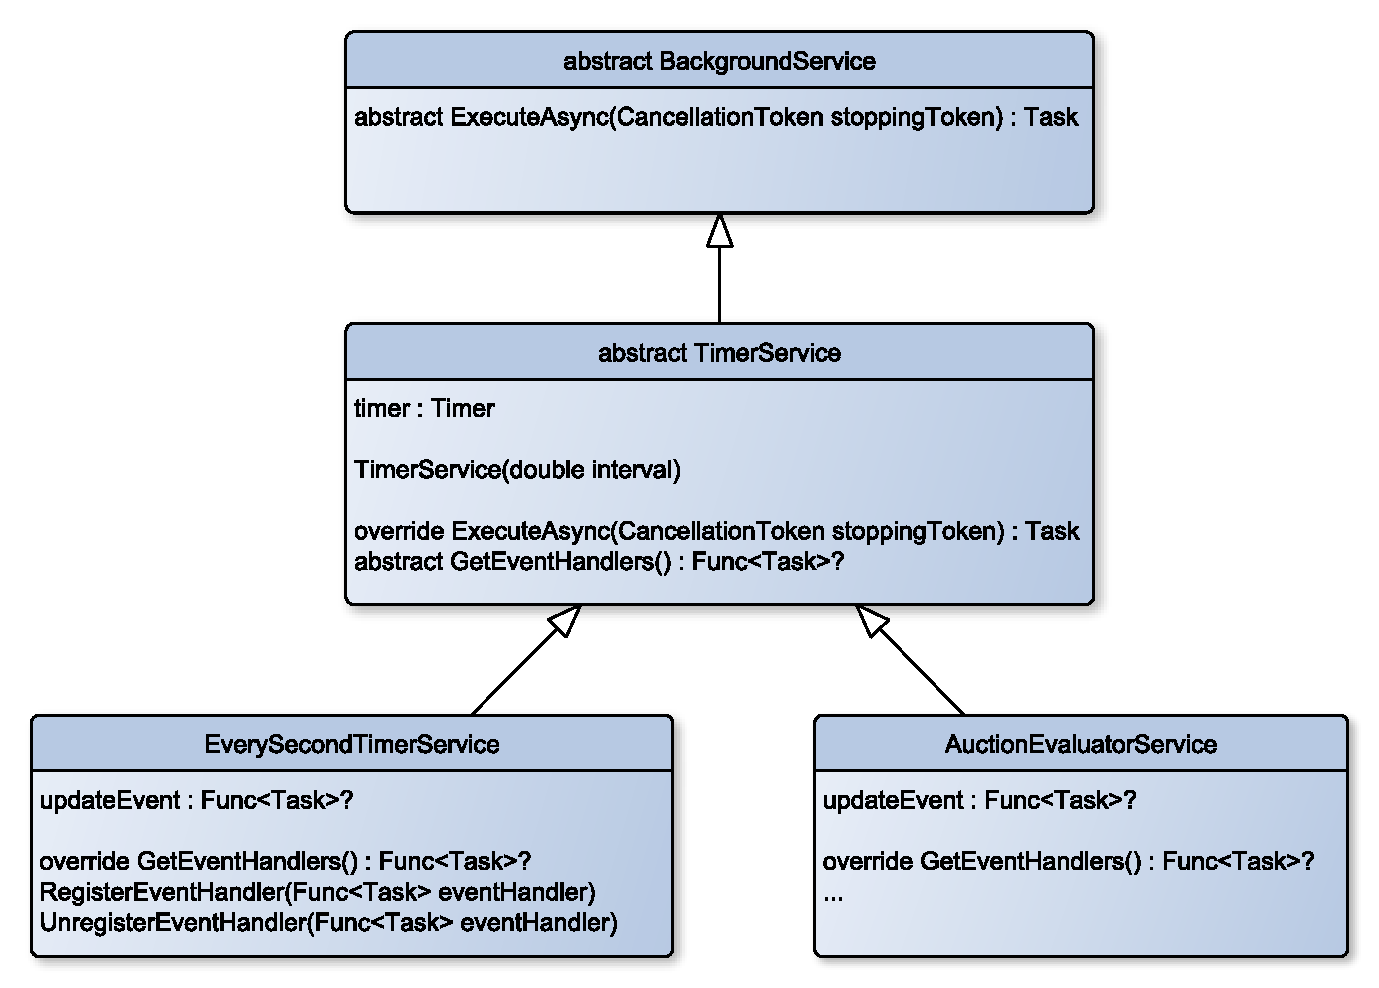
\includegraphics[width=140mm]{../img/timer services uml}
\caption{Časové služby využívajúce triedu \texttt{Timer}.}
\label{timer services uml}
\end{figure}

Interval by sa mohol predať potomkami prostredníctom parametra konštruktora triedy~\verb|TimerService| a pomocou abstraktnej metódy \verb|GetEventHandlers| triedy~\verb|TimerService| by si potomkovia mohli zadefinovať čo sa má diať. Takže v prípade triedy \verb|EverySecondTimerService| by to bolo prepočítanie a~prekreslenie odpočtu (resp.~zavolanie registrovaných metód) a~v~prípade triedy~\verb|AuctionEvaluatorService| by to bolo prejdenie aukčných ponúk a~vyhodnotenie tých ktoré by boli neaktívne.

Ďalej je potrebné si uvedomiť, že kód oboch služieb (\verb|EverySecondTimerService| a~\verb|AuctionEvaluatorService|) musí bežať na~pozadí v~osobitnom vlákne, aby neblokoval program a~neznepríjemňoval tým užívateľovi prácu s~aplikáciou. Pre implementáciu kódu bežiaceho na~pozadí nám .NET poskytuje viacero možností, pre naše účely by sa hodili napr.~rozhranie \texttt{HostedService}~\cite{hosted service} alebo~trieda~\texttt{BackgroundService}~\cite{background service}. Pre~naše účely by sa dali využiť obe možnosti, no trieda~\verb|BackgroundService| je určená pre~dlhotrvajúce úlohy bežiace na~pozadí~\cite{background service for long running tasks}, navyše autorovi vyhovuje viac možnosť s~triedou \verb|BackgroundService|, preto použijeme túto možnosť, a~to tak, že trieda \verb|TimerService| bude dediť od~triedy~\verb|BackgroundService|.

Trieda \verb|TimerService| zdedí od~triedy~\verb|BackgroundService| abstraktnú metódu~\verb|ExecuteAsync|~\cite{executeasync}. V~triede~\verb|TimerService| by sme ju mohli naimplementovať tak, že po~zavolaní by sa inicializovala inštancia triedy~\verb|Timer|, na~ktorej by sa zavolala metóda \texttt{Start}~\cite{start}. Inicializácia by spočítavala v~tom, že na~udalosť~\verb|Elapsed|~\cite{elapsed} inštancie triedy~\verb|Timer| by sa zaregstrovali metódy (obsluhy udalostí) definované v~potomkoch, tie vieme získať pomocou metódy \verb|GetEventHandlers| (ktorú sme spomenuli skôr v~texte). Ďalej nám už len stačí registrovať služby \verb|EverySecondTimerService| a~\verb|AuctionEvaluatorService| pomocou metódy \verb|AddHostedService| (viac informácií o~implementácii služieb bežiacich na~pozadí môžeme nájsť v~dokumentácii~\cite{addhostedservice}). Potom po~spustení aplikácie a~registrácií služieb sa už framework postará o~zavolanie našej implementácie metódy \verb|ExecuteAsync| (a~tým spustí na~pozadí naše služby).
